\begin{enumerate}
    \item  
   $$ w(t)h^h_t(t)=c^h_t+l^h(t)+k^h(t+1)$$
   Aggregate the constraint
   $$(1-\theta)K(t)^\theta H^{1-\theta}=\frac{1-\theta}{1+\beta}K(t)^\theta H^{1-\theta}+k(t+1)$$
   Note: $1-\frac{1}{1+\beta}=\frac{\beta}{1+\beta}$
   $$K(t+1)=\frac{\beta}{1+\beta}(1-\theta)K(t)^\theta H(t)^{1-\theta}$$
   $$k(t+1)=\frac{\beta}{1+\beta}\frac{1-\theta}{1+n}k(t)^\theta$$
   finding the steady state:
    $$k(t+1)=\frac{.98}{1.98}\frac{.67}{1.01}k(t)^{.33}=g(k(t))$$
     $$\bar{k}=0.3283\Bar{k}^{.33}$$
     $$\bar{k}=0.189$$
     \item figure
     \begin{figure}[H]
        \centering
        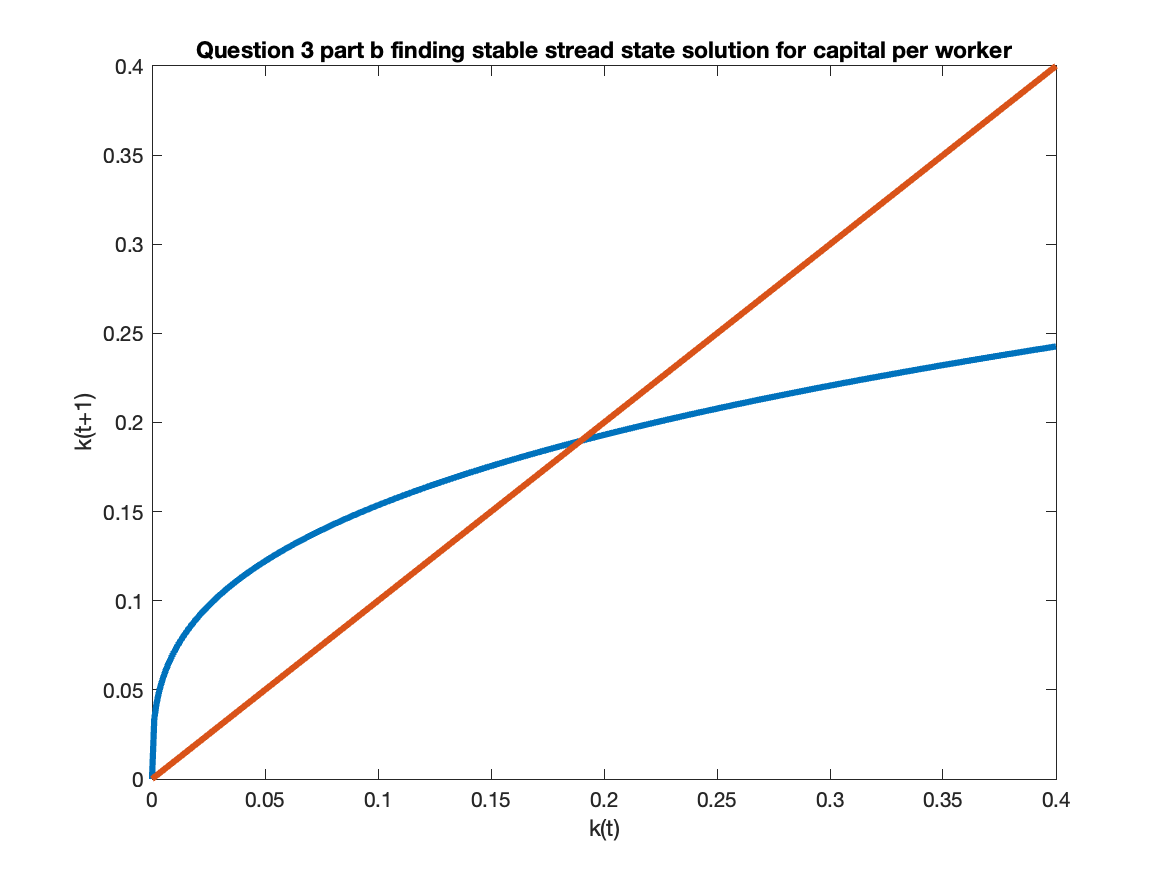
\includegraphics[width =.75\linewidth]{HW2/pics/HW1_Q3_b.png}
        \caption{finding stable steady state solution for capital per worker. This solution is stable as the k(t+1) is above the 45 degree line to the right and below the 45 degree line to the left}
    \end{figure}
    
         \item figure
     \begin{figure}[H]
        \centering
        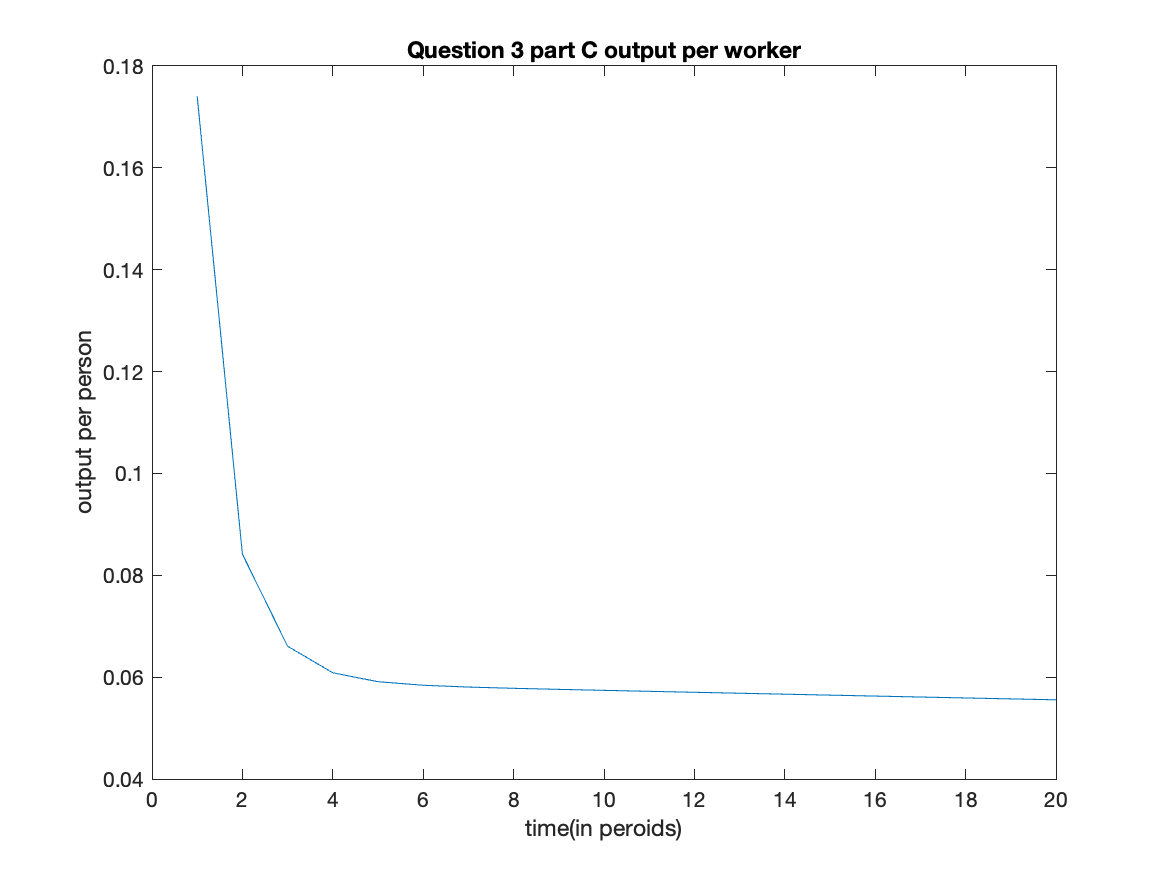
\includegraphics[width =.75\linewidth]{HW2/pics/HW1_Q3_c_output.png}
        \caption{"Output per worker"}
    \end{figure}

     \begin{figure}[H]
        \centering
        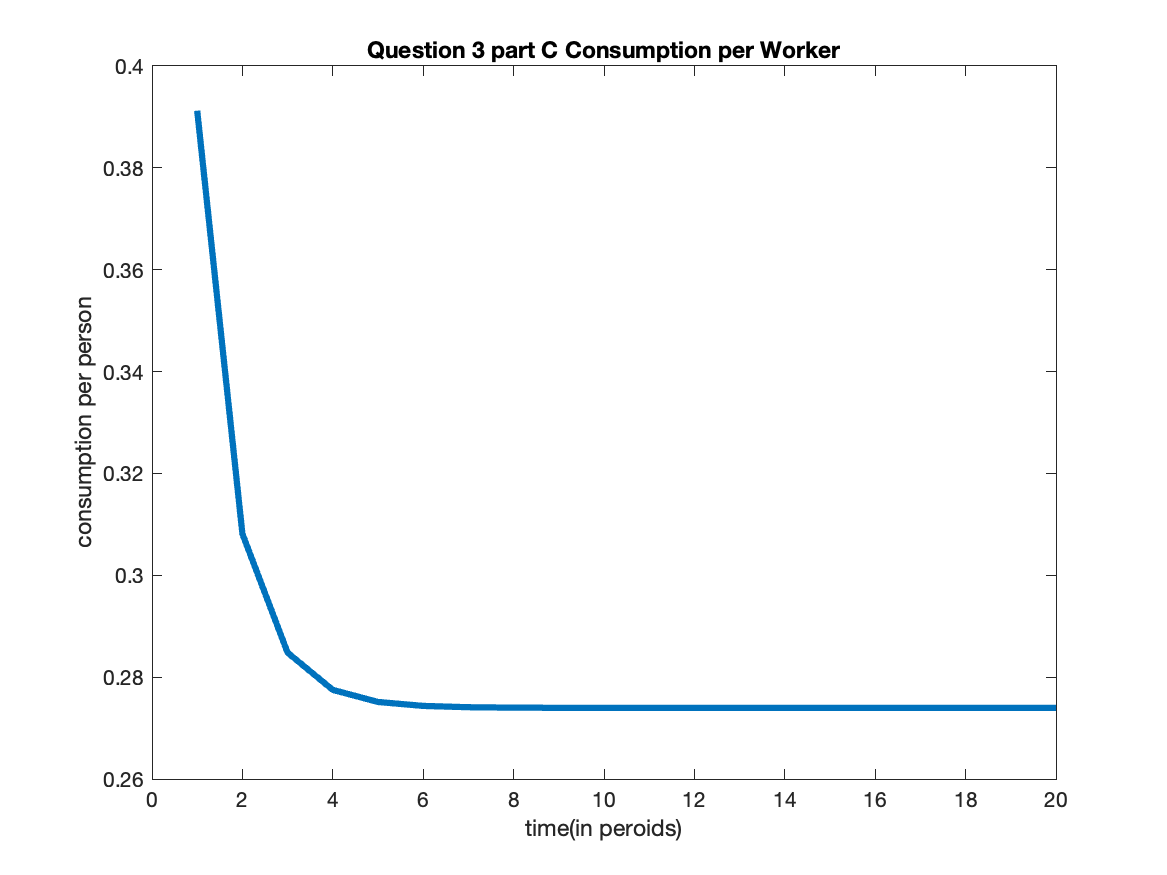
\includegraphics[width =.75\linewidth]{HW2/pics/HW1_Q3_c_consumption.png}
        \caption{"Consumption per worker"}
    \end{figure}
\end{enumerate}

the economy appear to converge to a steady state really quickly (only a few periods!). I think this is mostly a result of deprecation rate of capital is so high (all capital is replaced each period). As such it does not take as much time because there is less of an effect from the capital stock.